\documentclass[a4paper]{article}
\usepackage{graphicx}
\usepackage{xcolor}
\usepackage{url}
\usepackage{outlines}
\usepackage{listings}
\lstset{basicstyle=\ttfamily,
	showstringspaces=false,
	commentstyle=\color{blue},
	keywordstyle=\color{pink}
}
\lstset{emph={
	nc,tcp,udp,http,},emphstyle=\color{purple}
}
\usepackage{fancyhdr}
\usepackage{geometry}
\geometry{
	a4paper,
	total={170mm,257mm},
	left=20mm,
	top=20mm,
	bottom=39mm,
}

\setlength{\headheight}{82.70538pt}

\fancypagestyle{oida}{
	\fancyhf{}
	\fancyhead[L]{\fontsize{7.5}{7.5}htl donaustadt\\ Donaustadtstraße 45\\
		1220 Wien\\~\\ Abteilung: Informationstechnologie\\ 
	Schwerpunkt: Netzwerktechnik}
	\fancyhead[R]{
\includegraphics[scale=0.45]{images/logo.png}}

	\fancyfoot[L]{\today}
	\fancyfoot[C]{\jobname}
	\fancyfoot[R]{Seite: \thepage}
}

\begin{document}
\bibliographystyle{plain}
\pagestyle{oida}
\section*{Thema}
\par\noindent\rule{\textwidth}{0.4pt}

Laborprotokoll
TCP-UPD Header Verleich

\begin{figure}[h]
	
\includegraphics[scale=0.3]{images/meme.jpeg}
	\caption{memes klauen ist nicht ethisch}
\end{figure}

\vspace*{\fill}
Unterrichtsgegenstand:	NWT1|ZIVK

Jahrgang:	2BHIT

Name:	Stefan Fürst, Marcel Raichle

Betreuer: 	ZIVK

Übungsdaten:	24.5.2024, 31.5.2024,7.6.2024

Abgabedatum:	7.6.2024


\newpage
\tableofcontents

\newpage

\section{Aufgabenstellung}
Zussamenfassung der Aufgabenstellung von Cat-gpt:
% Meow, meow, darling, let me break it down for you in a sassy feline way:
\begin{enumerate}
	\item
	      Work in groups of 2, each with their own PC and Virtual Box with Kali Linux. Make sure network settings are correct and virtual machines have IP addresses. Verify with a ping. Start Wireshark and record the ping. You'll need to capture other transmissions too. Document every step in a log.
	\item
	      Use netcat to start a TCP server on port 5000. Connect with your partner using netcat. Document with screenshots and Wireshark. Answer questions about TCP connections and flags. Find and document TCP header fields. Document what happens when the server is closed.
	\item
	      Use netcat to start a UDP server on port 5000. Connect with your partner, document with screenshots and Wireshark. Answer questions about UDP connections and headers. Document server closure process.
	\item
	      Research TCP and UDP headers. Show and describe the most important fields in a one-page document. Compare header sizes and differences between TCP and UDP headers.
	\item
	      Bonus: Document how TCP and UDP are recorded in Wireshark. Research how port addresses are displayed. Show which Wireshark filters to use.
\end{enumerate}

% Now, go ahead and tackle these tasks like the curious cat you are! Meow!




\section{Zusammenfassung}
Netcad um einen TCP/UPD Server starten, mit Netcad verbinden und mit Wireshark die Verbindungen analysieren.


\newpage

\section{Übungsdurchführung}

\subsection{Aufsetzen der Server}
%command für das ding mit code block schön machen
\paragraph{TCP}
\begin{lstlisting}[language=bash,caption={Commands}]
# TCP
nc -l -p 5000
# UDP
nc -l -u -p 5000
\end{lstlisting}

\subsubsection{Verbinden mit dem Sever (TCP)}
nc 10.23.38.117 4201
\subsubsection{TCP-Verbindungsaufbau}
\begin{figure}[h]
	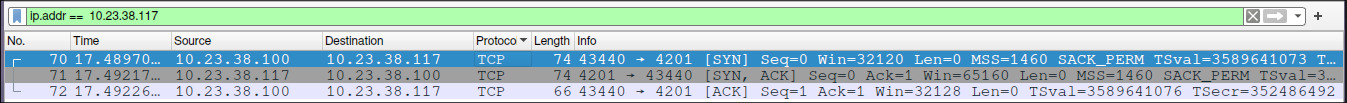
\includegraphics[scale=0.3]{images/handshake.jpeg}
	\caption{TCP 3 Way Handshake}
\end{figure}
\subsubsection{Nachrichten verschicken und empfangen}
\begin{figure}[h]
	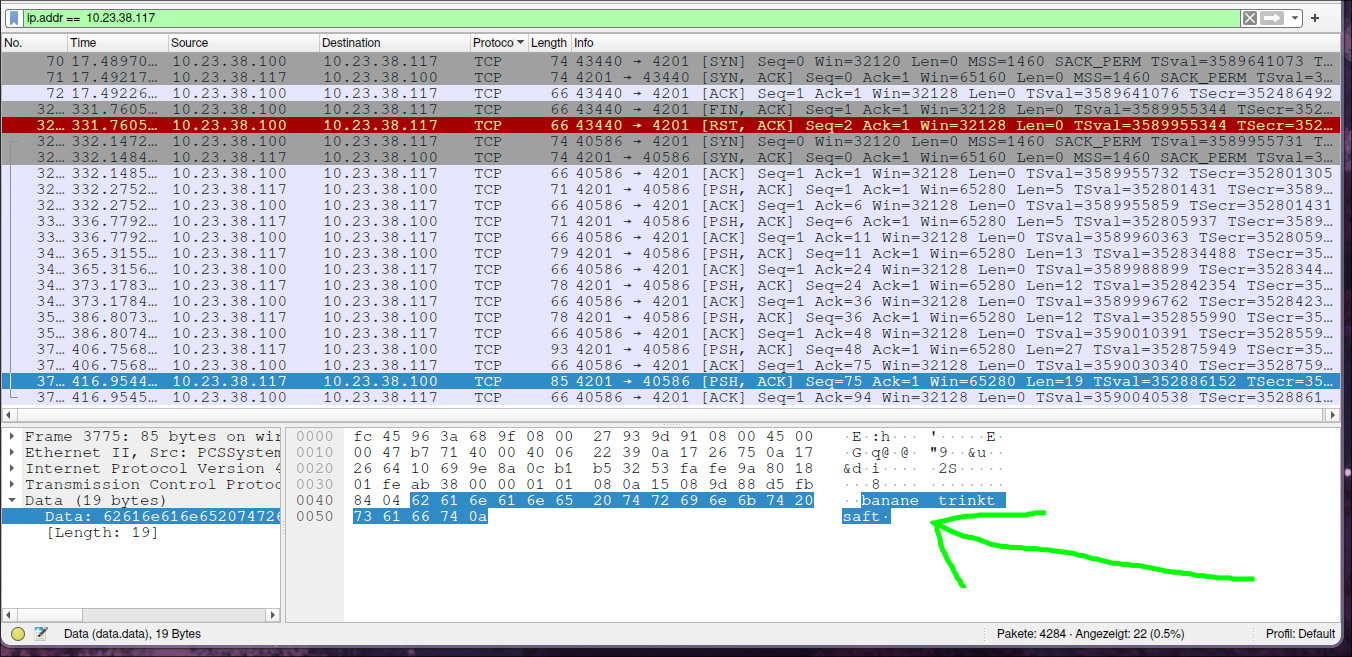
\includegraphics[scale=0.3]{images/nachricht.jpeg}
	\caption{Nachricht}
\end{figure}
\newpage
\subsubsection{TCP-Flags}
% https://www.geeksforgeeks.org/tcp-flags/
% den schaß citen
TCP-Flags dienen dazu um den Zustand, oder andere zusätzliche Informationen der Verbindung anzuzeigen.\\
Diese diesen zum Troubleshooten.
In der Übung ist die Push flag gesetzt, was bedeuted, dass die Nachricht sofort übertragen wird, ohne darauf zu warten, dass zusätliche Informationen auf der Senderseite gebuffert werden.\cite{TCP-Flags}
\\ Wird oft in Echtzeitapplikation benutzt.
\begin{figure}[h]
	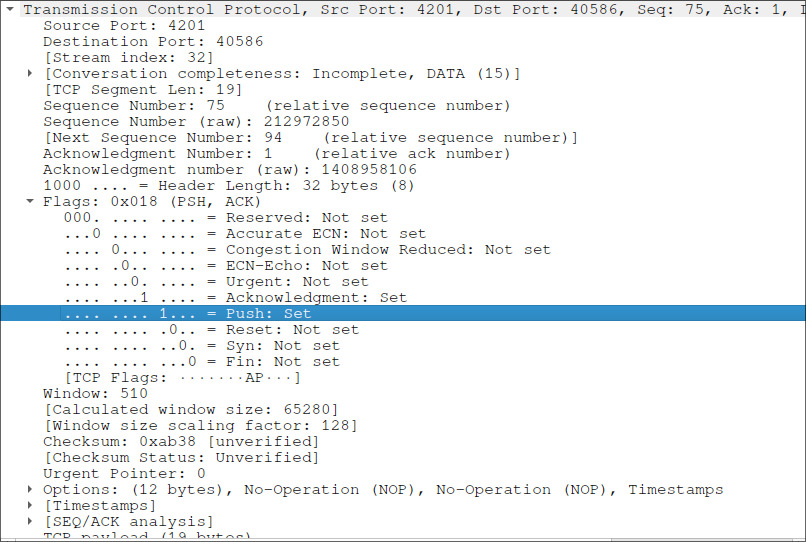
\includegraphics[scale=0.5]{images/tcp-flags.jpeg}
	\caption{TCP-Flags}
\end{figure}
\newpage
\subsubsection{TCP-Header}
%https://networklessons.com/cisco/ccie-routing-switching-written/tcp-header
Vorhandenen Felder
\begin{outline}
	\1 Source Port
	\1 Destination Port
	\1 Sequence Number
	\2 Zeigt an wie viele Daten in der TCP Session übertragen werden.
	\1 Acknowledgment Number
	\2 Vom Empfänger benutzt um das Nächste TCP Segment anzufordern
\end{outline}
Nicht Vorhandene Felder
\begin{outline}
	\1 Window
	\2 Gibt an wie viele bytes die der Empfänger empfangen will. Wird genutzt damit der Empfänger sagen kann, dass er mehr Daten empfagen will.
	\1 RSV
	\2 3 Reservierte Bits, die immer 0 sind.
	\1 Urgent Pointer
	\2 Wenn die URG-Flag gesetzt ist, zeigt dieser Pointer an, wo die Urgent Daten enden.
	\1 DO
	\2 Länge des Headers.
	\1 Flags
	\2 Vorher bereits erklärt.
	\1 Checksum
	\2 Benutzt für eine Prüfsumme um sicherzugehen, dass der TCP header korrekt is.
\end{outline}
\cite{TCP-Header}
\begin{figure}[h]
	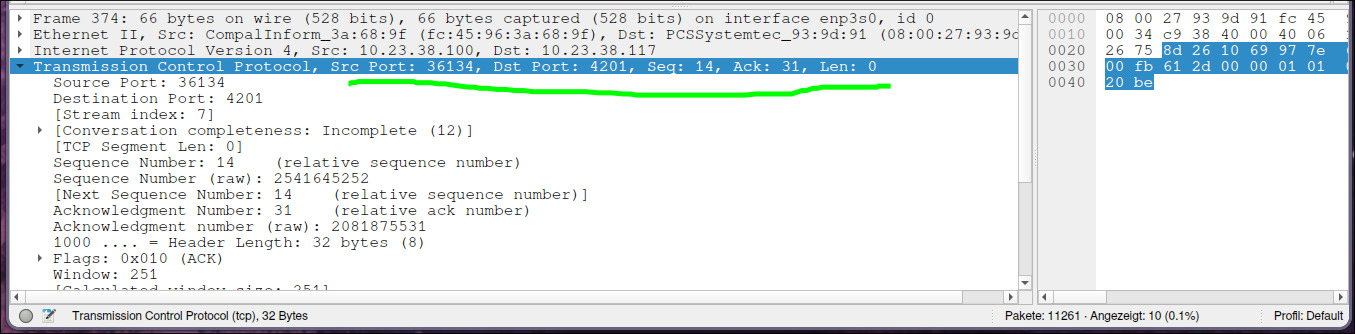
\includegraphics[scale=0.2]{images/tcp-header.jpeg}
	\caption{TCP-Header}
\end{figure}
\newpage
\subsubsection{Verbindungsabbruch}
\begin{figure}[ht]
	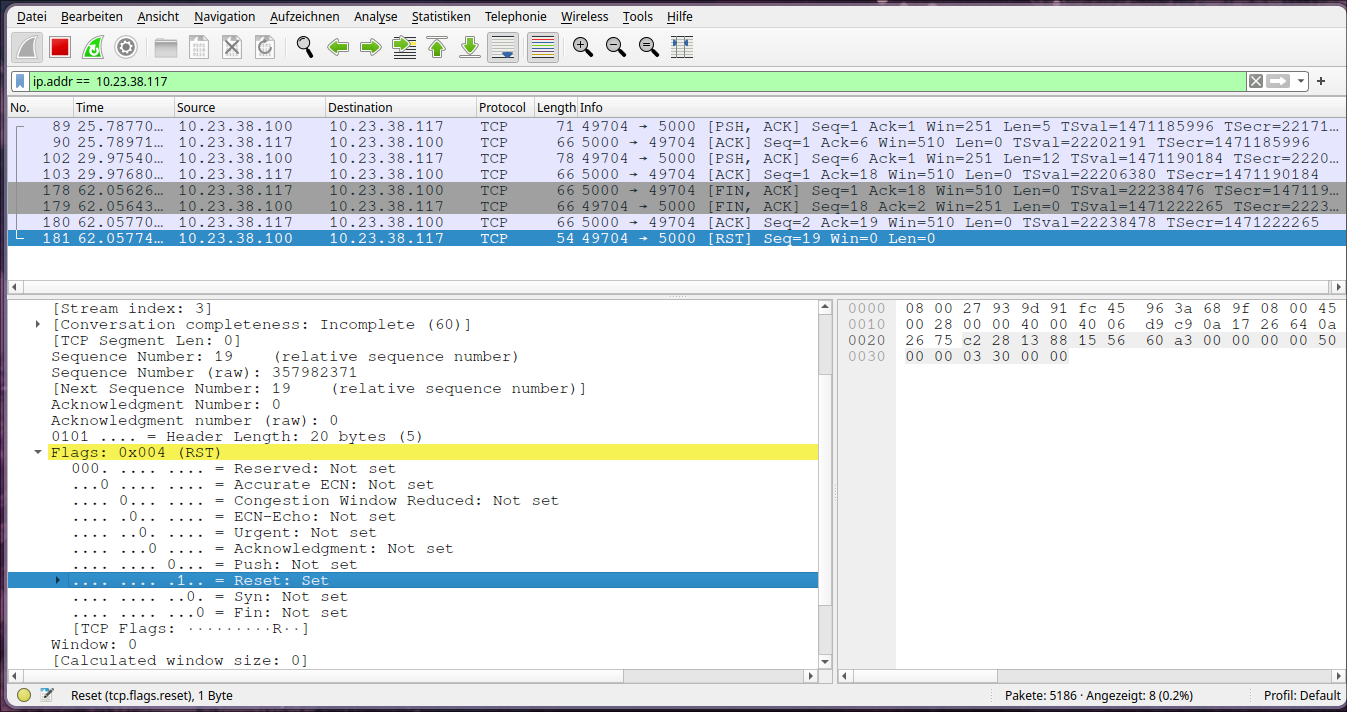
\includegraphics[scale=0.2]{images/verbindungsabbruch.png}
	\caption{Verbindungsabbruch}
\end{figure}

Die TCP-Flag Reset wird im Packet gesetzt und dann ist die Verbindung mit diesem Packet beendet.
\subsubsection{Verbinden mit dem Sever (UDP)}
nc -u 10.23.38.117 4201
\subsubsection{UDP-Verbindungsaufbau}
\begin{figure}[h]
	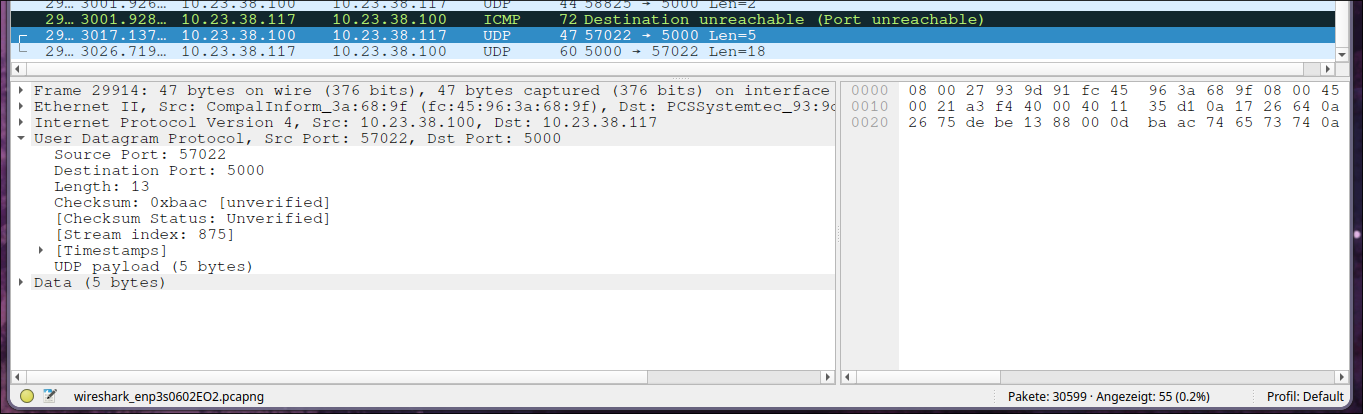
\includegraphics[scale=0.3]{images/udpverbindungsaufbau.png}
	\caption{UDP-Verbindungsaufbau}
\end{figure}

Im gegensatz zu TCP gibt es hier keinen 3-Way-Handsake und die Verbindung beginnt direkt.
\subsubsection{UDP-Nachrichten}
\begin{figure}[h]
	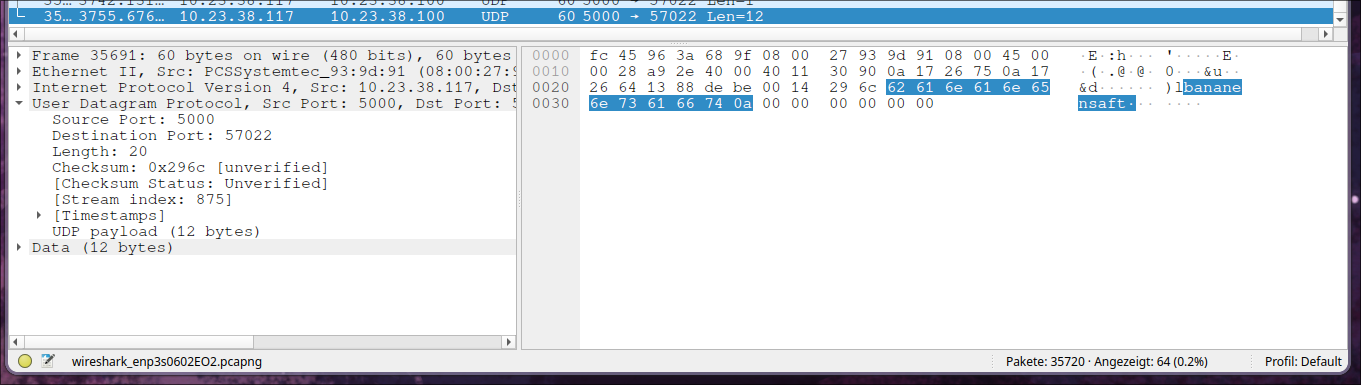
\includegraphics[scale=0.3]{images/udp-nachricht.png}
	\caption{UDP-Nachricht}
\end{figure}
\subsubsection {UDP-Header}
%https://de.wikipedia.org/wiki/User_Datagram_Protocol
\begin{outline}
	\1 Source Port
	\1 Destination Port
	\1 Länge
	\1 Checksum
\end{outline}
Diese Felder haben die selben bedeutungen wie bei TCP. \cite{UDP}
\\
\begin{figure}[h]
	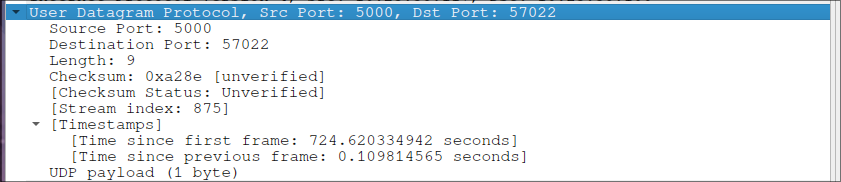
\includegraphics[scale=0.45]{images/UDP-Header.png}
	\caption{UDP-Header}
\end{figure}
\subsubsection{UDP-Verbindungsabbruch}
\begin{figure}[h]
	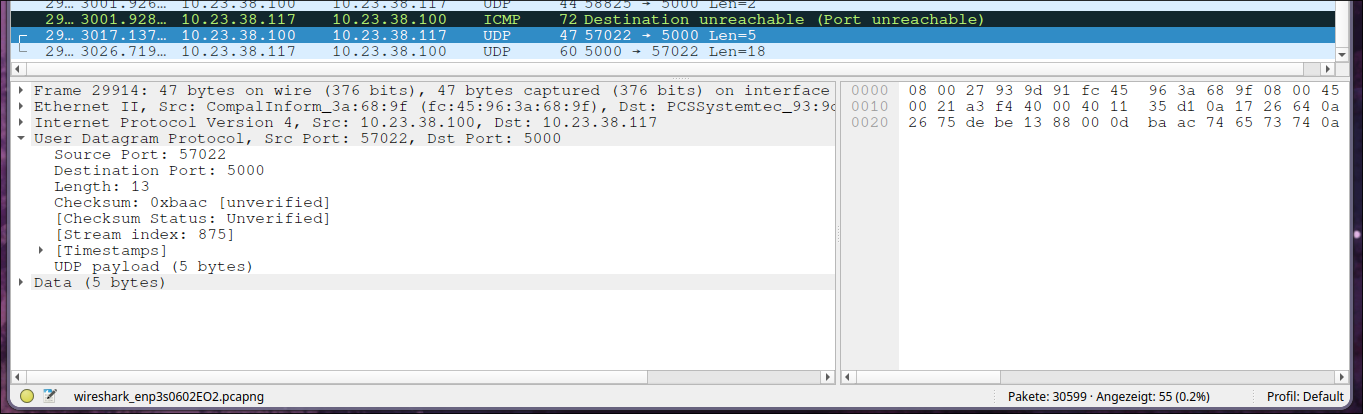
\includegraphics[scale=0.3]{images/udpverbindungsaufbau.png}
	\caption{UDP-Verbindungsabbruch}
\end{figure}

Die Verbindung endet einfach und es wird kein Packet zum Beenden der Verbindung geschickt.

\newpage
\subsection{TCP und UDP Headervergleich}

Im gegensatz zu TCP, UDP hat weniger Felder, da extra Felder wie Window, Sequnece und Achknowledgment Number einfach nicht benötigt, da der Sinn von UDP es ist, weniger overhead zu haben, damit eine schnellere Übertragung möglich ist.
\\
Der TCP-Header hat eine Minimale größe ein 20 Bytes, während der UDP-Header immer 8 Bytes groß ist. \cite{TCP-Header}\cite{UDP2}
\\
UDP hat nur die nur die Esenziellsten Felder, die benögtigt werden um eine Kommunikation durchzuführen.
\\
Wichtigste Felder:
\begin{outline}
	\1 Src/Destination Port
	\2 Ohne diesem Feld kann kommunikation nicht funktionieren.
	\1 Checksum
	\2 Wichtig um sicherzugehen, dass das Packet nicht Korrupt ist.
\end{outline}
\begin{figure}[h]
	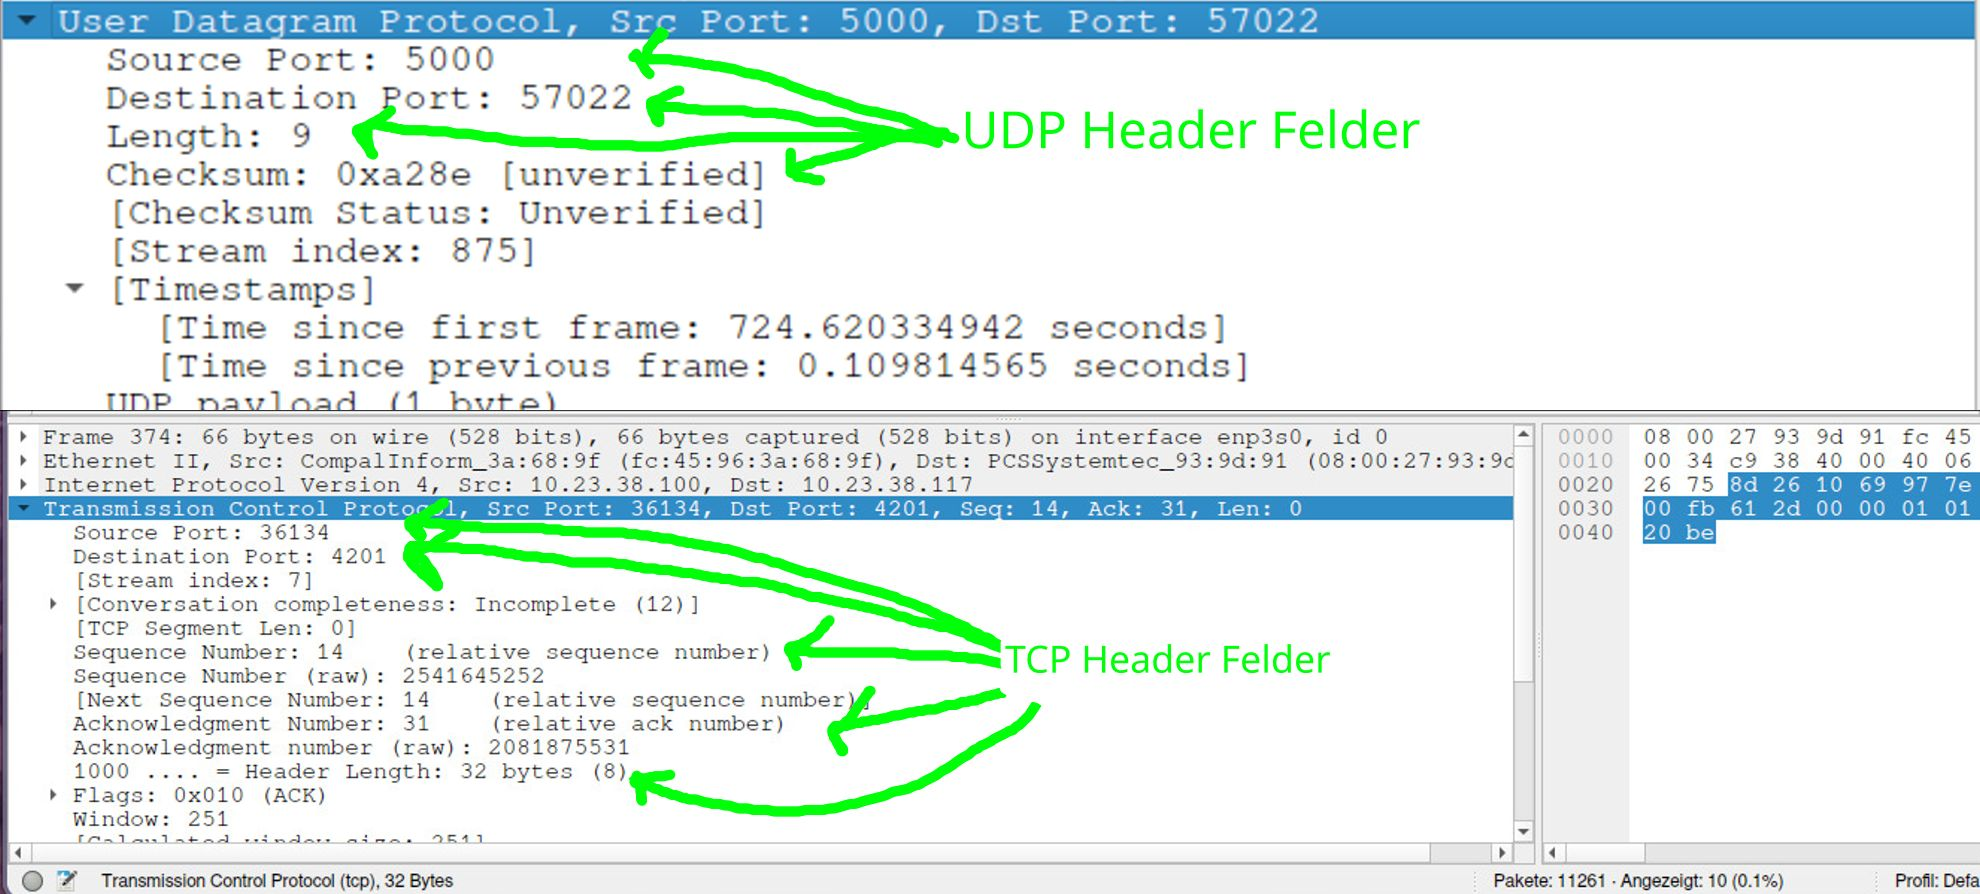
\includegraphics[scale=0.9]{images/vergleich.jpg}
	\caption{Header Vergleich}
\end{figure}

\subsection{Nach Ports filtern}
Nur Nach Port filtern:
\\
Protokoll.port == port
\\
Logische Operatoren können für komplexere Filter angewandt werden\cite{Portsfiltern}
\begin{lstlisting}[language=bash,caption={Commands}]
# tcp port 80 oder udp port 80
tcp.port == 80 || udp.port == 80

# auf port 80 nach verlorenen tcp segmenten filtern
tcp.port == 80 && tcp.analysis.lost_segment
\end{lstlisting}

\newpage
\section{Quellen}
\bibliography{quellen}
\newpage
\section{Abbildungsverzeichnis}

\listoffigures

\end{document}
